\documentclass[11pt]{article}
\usepackage[letterpaper,margin=1in]{geometry}
\usepackage[T1]{fontenc}
\usepackage[utf8]{inputenc}
\usepackage{lmodern}
\usepackage{graphicx}
\usepackage{amsmath,amssymb}
\usepackage{booktabs}
\usepackage{caption}
\usepackage{hyperref}

\title{KOP Homework 01}
\author{krausri1@fit.cvut.cz}
\date{November 2025}

\begin{document}
\maketitle

\section*{Executive Summary}
ProbSAT beats GSAT on every metric (success rate, PAR10, flip count distribution).

\section{Introduction}
We set out to compare the two SAT algorithms, GSAT and ProbSAT, on our set of data.
The better algorithm should converge faster, especially on larger instances.

\section{Methods}
\subsection{Solvers}
We used the GSAT implementation from \href{https://courses.fit.cvut.cz/NI-KOP/download/index.html}{Course Pages} with a fixed parameter $p=0.4$.

The probSAT solver was downloaded from \href{https://github.com/adrianopolus/probSAT}{Adrian Balint's GitHub}
and modified to return results in the same format as our GSAT implementation.
Fixed parameters:
\(
c_m = 0,
c_b = 2.3
\).

\subsection{Instances}
We chose to use the ''ruf'' set of instances from \href{https://courses.fit.cvut.cz/NI-KOP/download/index.html}{Course Pages}.
Specifically: ruf20-91, ruf36-157, ruf50-218, ruf75-320.

\subsection{Experiment}
To test the solvers, each solver was run $1\,000$ times per configuration.
Each instance contains $1\,000$ configurations.
In total, we tested $8\,000\,000$ solver runs.

The max\_flips parameter was set to $10\,000$ for all runs.

\subsection{Measurements}
For each experiment run, we saved the number of flips,
whether the run was successful, the instance and configuration name,
and the solver used. The cap was $10\,000$ flips, so unfinished runs always
report $10\,000$ flips.

\subsection{Implementation}
The python implementation creates subprocesses which call the GSAT and ProbSAT binaries, which are run in parallel.
It then aggregates all results into a single pandas dataframe.
The dataframe is then saved and further processed in a marimo notebook to create the tables and figures.

To run the experiments, we used Metacentrum. The final experiment was run on a 32-core AMD Ryzen CPU, the run took roughly 1 hour.

\subsection{Metrics}
All tables and plots derive from the following metrics:
\begin{itemize}
  \item \textbf{Success rate}: share of runs that satisfied all clauses.
  \item \textbf{PAR10}: penalized average runtime, calculated as mean flip count where each failed run is penalised by a factor of 10 ($10\times10\,000$ flips). This metric favours solvers that finish often and quickly.
  \item \textbf{Log-normal parameters}: mean and standard deviation of $\log(1+\text{flips})$ across all runs, lower values imply faster and more concentrated performance. The metric makes sense under the assumption that the number of flips comes from a log-normal distribution.
  \item \textbf{Flip-count histogram}: visualization of flip-count distribution (both linear and log scale). Only successful runs are visualized because otherwise unsuccessful runs would saturate the histogram at the max\_flips value and the actual flip count is unknown.
  \item \textbf{Empirical CDFs}: CDF of flips for successful runs, corrected ''CDF'' scaled by the success probability, making it reflect performance over all runs.
\end{itemize}


\section{Results \& Discussion}
ProbSAT yields better results over all metrics.

Success rate (\autoref{tab:success}) is slightly in favor of ProbSAT, expecially for the largest instance, where it clearly dominates.

ProbSAT yields significantly lower PAR10 scores (\autoref{tab:par10}).

Both mean and standard deviation of $\log(1+flips)$ (\autoref{tab:logmean}, \autoref{tab:logstd}) are lower for ProbSAT,
indicating faster convergence and greater stability.

The histogram of flip counts (\autoref{fig:hist}) shows that most of the problems are solved with a low number of flips,
but it is too saturated to make any conclusions about which solver is better.

However if we look at the histogram of $\log(1+flips)$ (\autoref{fig:loghist}),
we see that it is consistent with the mean and std measured earlier. We can clearly
see that ProbSAT is skewed left, towards lower flip counts.

In both CDFs (\autoref{fig:cdf},\autoref{fig:cdfcorr}), ProbSAT is above GSAT, indicating faster convergence.

\section{Conclusion}
ProbSAT is preferable to GSAT on the tested ruf instances.

\newpage
\section*{Tables}

\setlength{\tabcolsep}{9pt}
\begin{center}
  \begin{minipage}{0.48\textwidth}
    \captionof{table}{Success rate (\%), higher is better.}
    \label{tab:success}
    \begin{tabular}{lcc}
      \toprule
      dataset & GSAT & ProbSAT \\
      \midrule
      ruf20-91 & \textbf{100.00} & \textbf{100.00} \\
      ruf36-157 & 99.20 & \textbf{99.93} \\
      ruf50-218 & 96.18 & \textbf{99.37} \\
      ruf75-320 & 85.96 & \textbf{96.55} \\
      \bottomrule
    \end{tabular}
  \end{minipage}
  \hfill
  \begin{minipage}{0.48\textwidth}
    \captionof{table}{PAR10, lower is better.}
    \label{tab:par10}
    \begin{tabular}{lcc}
      \toprule
      dataset & GSAT & ProbSAT \\
      \midrule
      ruf20-91 & 161.00 & \textbf{94.00} \\
      ruf36-157 & 1401.00 & \textbf{404.00} \\
      ruf50-218 & 4914.00 & \textbf{1296.00} \\
      ruf75-320 & 15670.00 & \textbf{4717.00} \\
      \bottomrule
    \end{tabular}
  \end{minipage}
\end{center}

\vspace{1.2em}
\begin{center}
  \begin{minipage}{0.48\textwidth}
    \captionof{table}{Log-normal mean flips, lower is better.}
    \label{tab:logmean}
    \begin{tabular}{lcc}
      \toprule
      dataset & GSAT & ProbSAT \\
      \midrule
      ruf20-91 & 4.03 & \textbf{3.85} \\
      ruf36-157 & 5.36 & \textbf{5.01} \\
      ruf50-218 & 6.21 & \textbf{5.75} \\
      ruf75-320 & 7.15 & \textbf{6.59} \\
      \bottomrule
    \end{tabular}
  \end{minipage}
  \hfill
  \begin{minipage}{0.48\textwidth}
    \captionof{table}{Log-normal std of flips, lower is better.}
    \label{tab:logstd}
    \begin{tabular}{lcc}
      \toprule
      dataset & GSAT & ProbSAT \\
      \midrule
      ruf20-91 & 1.35 & \textbf{1.13} \\
      ruf36-157 & 1.51 & \textbf{1.22} \\
      ruf50-218 & 1.54 & \textbf{1.25} \\
      ruf75-320 & 1.47 & \textbf{1.27} \\
      \bottomrule
    \end{tabular}
  \end{minipage}
\end{center}

\section*{Figures}

\begin{figure}[htbp]
  \centering
  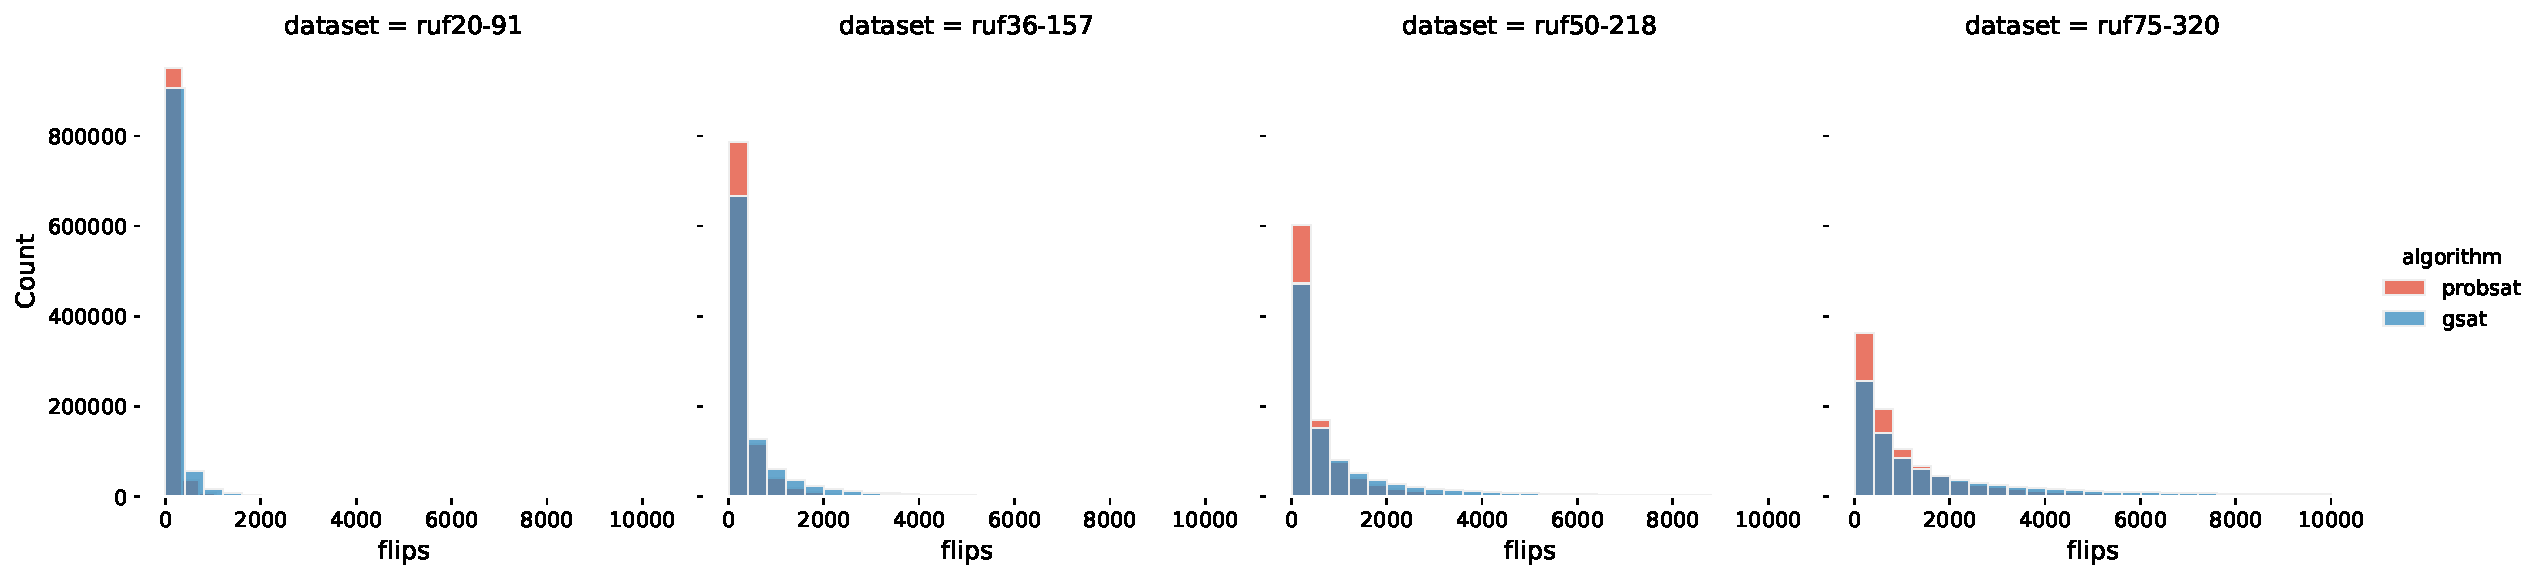
\includegraphics[width=\linewidth]{data/plots/hist.pdf}
  \caption{Histogram of flip counts for successful runs (linear scale).}
  \label{fig:hist}
\end{figure}

\begin{figure}[htbp]
  \centering
  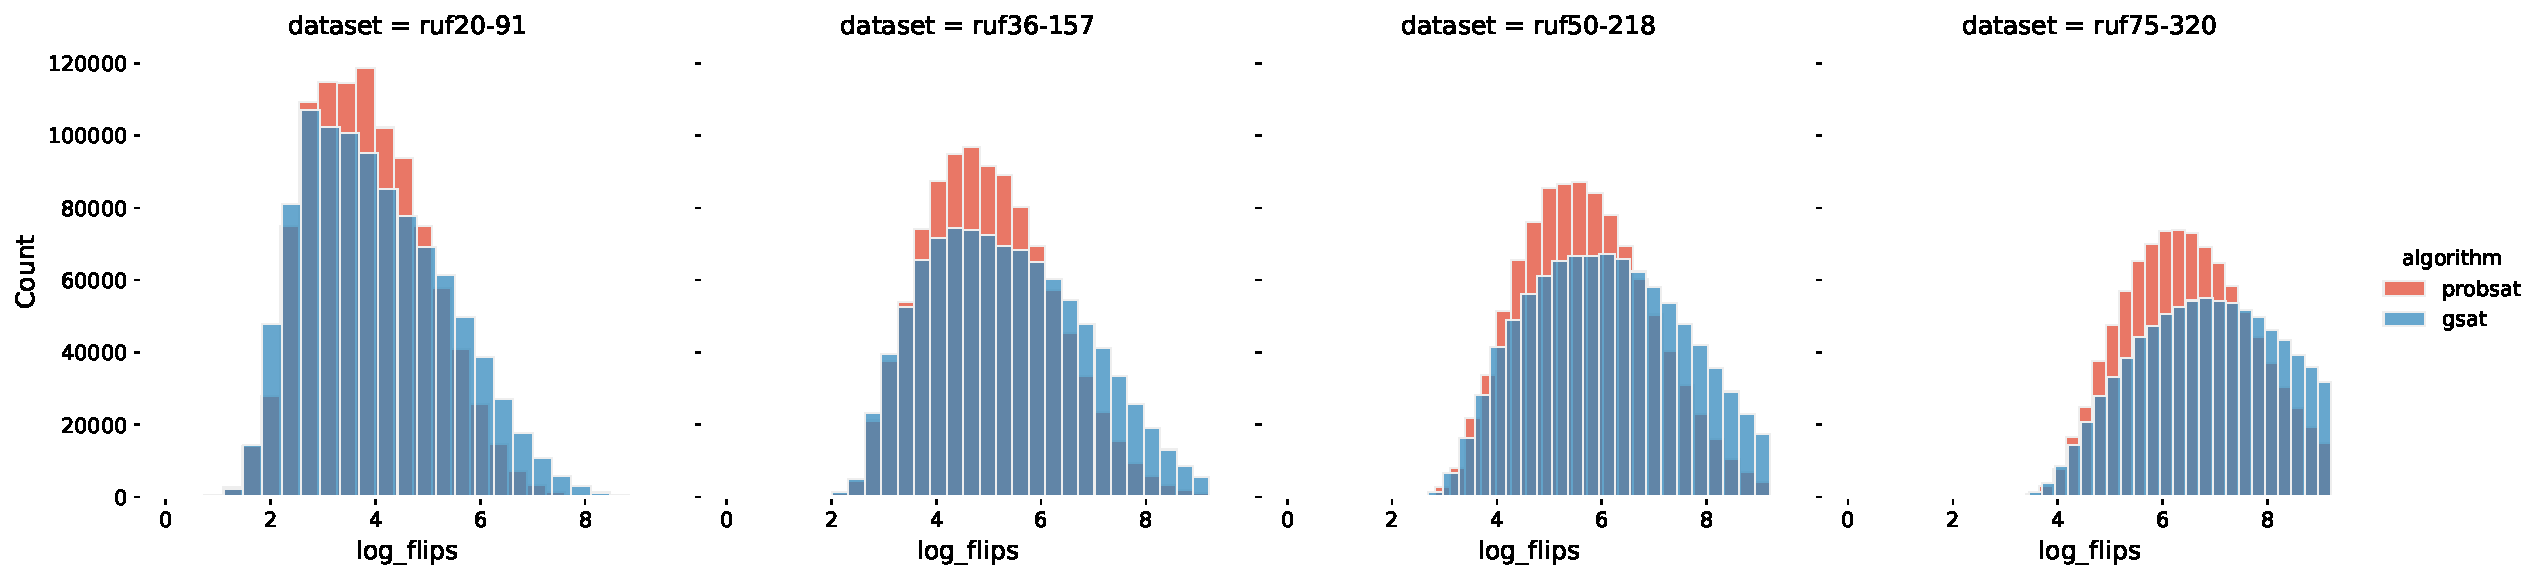
\includegraphics[width=\linewidth]{data/plots/log_hist.pdf}
  \caption{Histogram of flip counts for successful runs (log scale).}
  \label{fig:loghist}
\end{figure}

\begin{figure}[htbp]
  \centering
  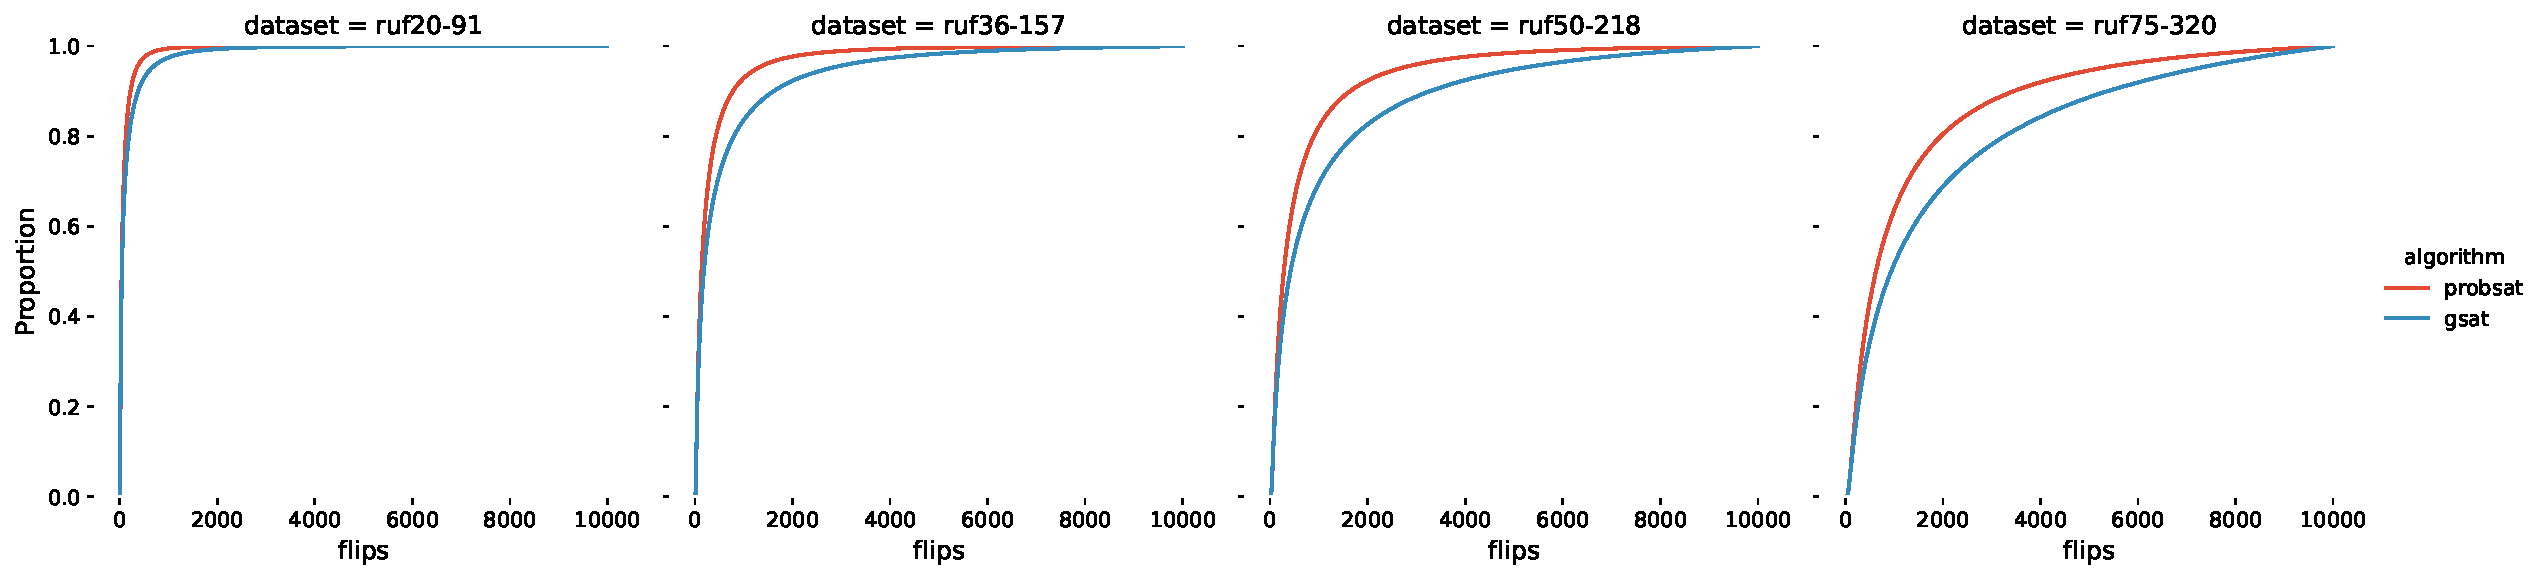
\includegraphics[width=\linewidth]{data/plots/cdf.pdf}
  \caption{Empirical CDF of flip counts for successful runs only.}
  \label{fig:cdf}
\end{figure}

\begin{figure}[htbp]
  \centering
  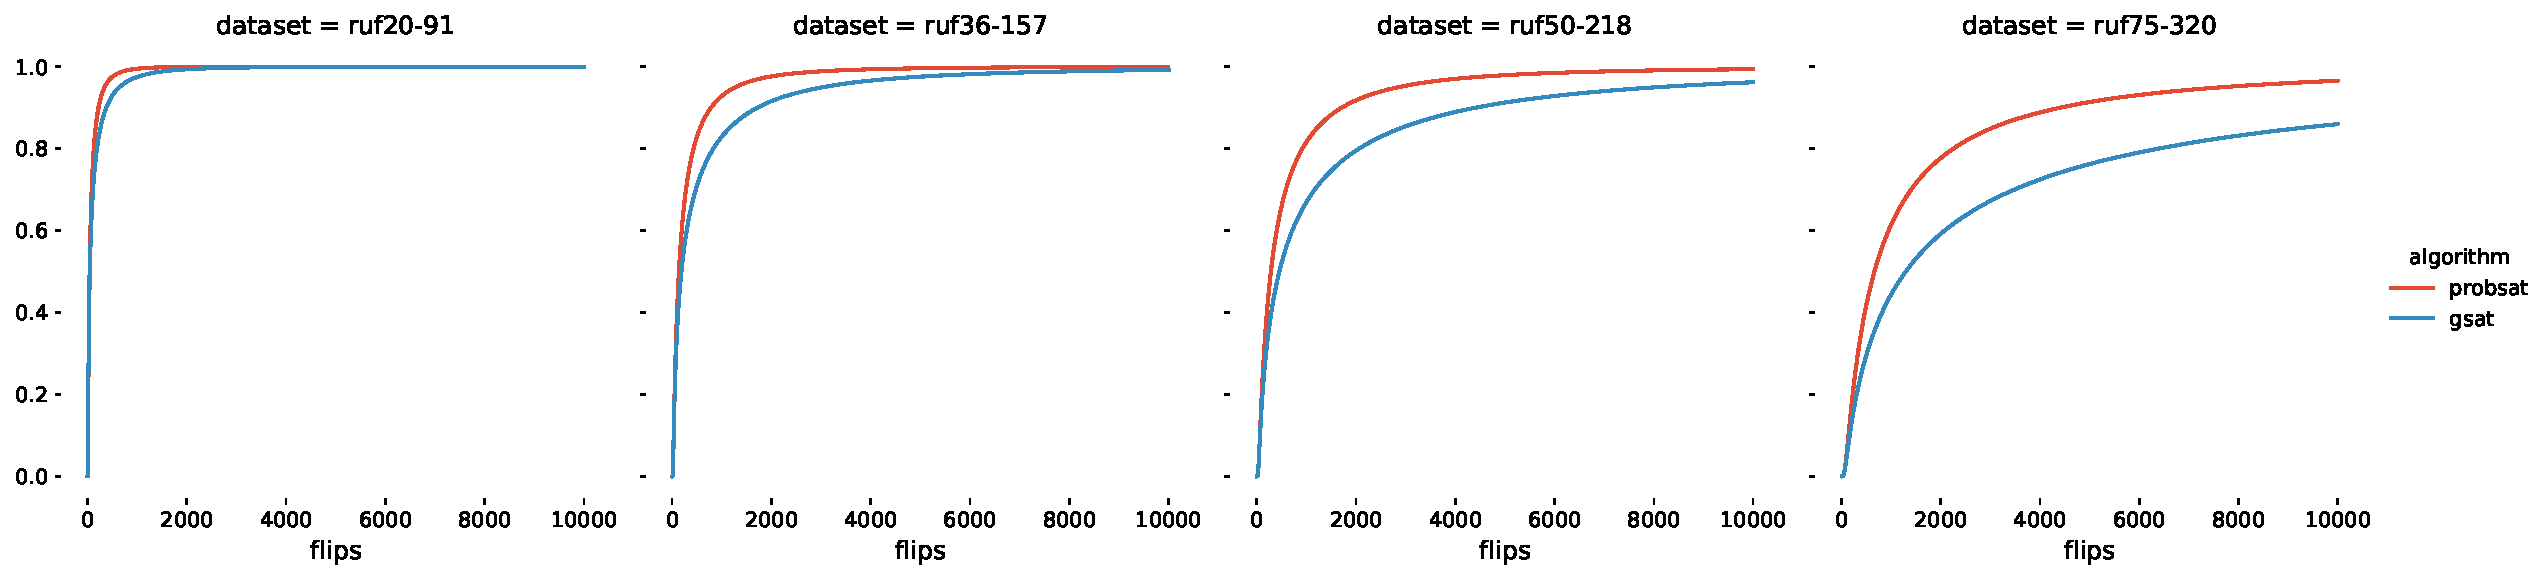
\includegraphics[width=\linewidth]{data/plots/cdf_corrected.pdf}
  \caption{Empirical CDF of flip counts over all runs (success-weighted correction for unfinished runs).}
  \label{fig:cdfcorr}
\end{figure}

\end{document}
